% !Mode:: "TeX:UTF-8"
%!TEX program  = xelatex

%\documentclass{cumcmthesis}
\documentclass[withoutpreface,bwprint]{cumcmthesis} %去掉封面与编号页
\usepackage{url}
\title{论文标题}
\tihao{A}
\baominghao{4321}
\schoolname{东南大学}
\membera{卢立强}
\memberb{喻泽弘}
\memberc{杜昕昱}
\supervisor{老师}
\yearinput{2019}
\monthinput{05}
\dayinput{11}

\begin{document}

 \maketitle
 \begin{abstract}

这里是摘要

\keywords{\quad  聚类分析\quad   \quad  }
\end{abstract}

%目录
\tableofcontents

\section{问题提出与重述}

\subsection{问题的提出}

随着互联网的整体升级与手机行业的迅速发展,移动支付也逐渐得到普及,受到用户与商家的青睐。移动支付即通过手机而非现金或银行卡完成支付,具有移动性,及时性,定制化,集成性等特点,发展前景巨大,应用领域丰富。其中公交移动支付可以解决现金支付,刷卡支付等带来的不便,也可减少人工成本。

在出行领域相比打车与共享单车,公交地铁的体量更大,交易量也十分可观,应用到移动支付行业也会带来大量利润,所以通过分析市民乘车的支付行为建立盈利模型来分析与估计支付平台的商业盈利十分必要。



\subsection{问题的重述}

1.通过附件1,2给出的某市部分公交支付的信息与数据说明,分析该市乘车人的支付行为特征。

2.参考附件3的信息,建立第三方支付平台的商业盈利数学模型,定量分析第三方平台的收支和盈利情况。

3.通过附件1,2给出的该市四分之一的公交与地铁安装移动支付设备后试营运期间数据,估计该市实现全部公交移动支付后第三方平台的盈利情况。


\section{问题分析}

\subsection{问题的分析}

\textbf{问题一分析:}

要对用户的支付行为特征进行分析,我们用统计与聚类分析两个方法提取用户的支付行为特征并进行分析。根据附件一二给出的公交支付信息,由于其中有缺失数据与错误数据,需要先进行数据清洗与数据填充,得到有效数据。先建立统计模型,通过建立哈希表对数据进行整理,对用户的支付行为分别从不同时间,不同个体等角度进行统计分析,得到统计数据,绘制出相应图表,根据图表与数据提取用户支付行为特征并尝试分析其原因。建立聚类分析模型,通过不同的用户标签区分用户,分析聚类结果得到用户支付行为特征。

\textbf{问题二分析 :}

附件三给出了第三方支付平台的盈利模式,了解到第三方支付平台有手续费,广告费,沉淀资金的利息收入,服务费等多种盈利模式。其中每个盈利模式都有自己的方案,通过对每个盈利模式的方案进行分析,可以分别得到每一部分收益的表达式。支出方面分为机器成本,维护成本与推广费用几个方面,通过对第三方平台在各个环节产生的支出进行分析可得出每一项支出的表达式。平台盈利即为平台收入减平台支出。构建好平台盈利模型,通过定量分析的方法更改影响模型的因素,绘制盈利变化的曲线,分析收支与盈利情况。

\textbf{问题三分析 :}

公交移动支付覆盖率从该市四分之一扩展到全部,会对客流量产生影响,进而影响第三方支付的盈利。针对客流量,可以通过一个城市的实例来找到客流量的比例,以南京市地铁为例,分析其中1/4线路与全部项目的客流量比例,得到占比数据,通过第一问得到的数据可以对移动支付全覆盖之后该市移动支付的人数进行估算,带入第二问建立的模型中得到盈利数据。从支付行为特征我们发现移动支付占比会随移动支付实施的时间发生变化,通过第一问数据可建立移动支付比例随时间增长的变化曲线,应用于第二问的模型中可建立覆盖率提升之后平台盈利随时间变化的曲线,即可估计与分析第三方平台在该市在移动支付全覆盖后的盈利情况。

\section{模型的假设}


\subsection{模型的假设}

\begin{itemize}
\item[(1)] 假设表中显示的支付时间均为有效时间,即乘客在支付时认为公交处于运营状态。
\item[(2)] 假设同一个人只能拥有一个ID。
\item[(3)] 假设移动支付试运营发生在该市客流量最大的$1/4$线路中
\item[(4)] 假设南京地铁的部分运营数据可以反映该市公共交通的运营数据 
\end{itemize}

\section{符号说明}
\begin{center}
\makeatletter\def\@captype{table}\makeatother
\begin{table}[htbp]
\small 
\centering
\caption{符号说明}\label{tab:aStrangeTable}\centering%添加标题 设置标签
\begin{tabular}{c|c|c}\hline
符号& 表示含义& 单位\\\hline
$SumCharge$ & 所有天数的公共交通支付笔数数目的总和 & \\
$SumCharge^{MobilePay}$ & 所有天数移动支付公共交通的成交量 & \\
%$MonthlyCharge_i$ & 第$i$月一周的公共交通支付数目的总和 &\\
%$MonthlyCharge^{MobilePay}_i$&第$i$月移动公共交通支付的笔数&\\
$DailyCharge_{(i,j)}$&第$i$月星期$j$的公共交通支付数目&\\
$DailyCharge^{MobilePay}_{(i,j)}$&第i月星期j当天移动支付公共交通的笔数&\\
%$\overline {times}$&人均乘车次数&\\
%$\overline {times_i}$&第$i$月人均乘车次数&\\
%$\overline {times}_{(i,j)}$&第$i$月星期$j$的人均乘车次数&\\
%$\overline {times}^{mobilePay}_{(i,j)}$&第$i$月星期$j$的人均移动支付公共交通笔数&\\
%$HourCharge_{i}$&一天第$i\sim i+1$小时内,公共交通的支付笔数&\\
%$HourCharge_{i}^{mobilePay}$&一天第$i\sim i+1$小时内,移动支付公共交通的笔数&\\
%$Uptime_{m}^{i}$&乘客$m$在时间段$i\sim i+1$的公交支付笔数, $0\leq i \leq 23$&\\
$CustomerSum(i)$&乘客$i$公共交通支付总量&\\
$CustomerSum(i)^{mobilePay}$&乘客$i$公共交通移动支付的数量&\\
$CustomerValidSum(i)$&乘客$i$有效公共交通支付总量&\\
$S_{sum}$&销售总额&\\RMB
$Pay_{sum}$&用户支付笔数&\\
$FreeRate$&第三方平台对用户的手续费率&\\
$ServiceRate$&第三方平台对商户的服务费率&\\
$adFree$&第三方平台向商户收取的广告费&RMB/CPM\\
$\overline {remain}$&用户人均余额&RMB\\
${NumberOfPeople}$&使用该第三方支付平台的人数&\\
$SedMoney(i)$&第i月的存入银行的沉淀资金&RMB\\
$SedMoney^j(i)$&第i月的沉淀资金经过$j$月以后的总额&RMB\\
$r=IncreaseRate$&沉淀资金的增长率&\\\hline
\end{tabular}
%\caption{这是一张三线表}\label{tab:aStrangeTable}  标题放在这里也是可以的
\end{table}
\end{center}



\section{模型建立与求解}
\subsection{问题一的建模与解答}
\subsubsection{数据清洗}
附件一,二给出了某市部分公交支付的信息与数据,分别取了2,5,8,11月份中连续的7天的支付信息,包括支付ID,上一次乘车交易时间,本次乘车时间,付款方式,当月地铁与公交乘车次数,与乘车总次数。每天大概有一百多万条乘车数据,而其中也有许多无效数据与错误数据,需要我们在统计前对数据进行清洗,现对数据进行以下三个方面的清洗:

1. 对于PAYTYPE值为Null的数据:将PAYTYPE项中的Null值替换为0。附件一中的PAYTYPE项表示的是支付方式,其中0代表公交移动支付,1代表公交卡支付,而通过刷卡记录的规则可知Null为没刷卡,所以将Null将NULL算为非公交卡支付。通过观测2月、5月、8月和11月的公交数据可以发现,除二月以外的其他月中,
支付类型只为0,1和NULL,又因为NULL表示非公交卡支付,所以这里我们可以把NULL归为移动支付。对于二月的数据,我们可以把支付类型为NULL的数据,按比例分配给移动支付方式和其它支付方式。

2.对于UPTIME没有记录的数据:UPTIME中的0001-1-1表示没有刷卡记录,对这部分数据进行填充:

(1)若该乘客相同的月份的相邻两次记录中,前一次的UPTIME丢失,而后一次的乘车记录给出了LASTTIME,则我们使用后一次记录的LastTtime填充上一次记录的UPTIME。

(2)若找不到可以补充的LASTTIME,则按照以下步骤填充:

Step1:将乘客$i$所有有效乘车时间提取出来,构成数组$Uptime_i$[k](k=0,1...CustomerValidSum(i))。

Step2:在0$\sim$CustomerValidSum(i)范围内随机生成数字n。

Step3:将n当作数组下标在$Uptime_i$数组中取$Uptime_i$[n]作为填充数据。

Step4:对于多个Uptime缺失的,重复Step2$\sim$Step4步骤

3. 清理极少乘坐公交的人:对于$CustomerSum(i)\leq2$ 的乘客信息,由于他们乘坐公交次数很少,支付行为特征难以分析,或者不是该市市民,对于这种乘客的信息进行清理,删掉这条ID相关的信息。

\subsubsection{数据统计}

由于支付数据量很大,我们先遍历一边所有excel表格,根据每个人的ID构建哈希表储存他们的信息,根据有效数据整理出如下数据:

(1)每天的移动支付笔数:$\overline {times}^{mobilePay}_{(i,j)}​$

(2)每天的公交支付笔数:$\overline {times}_{(i,j)}$

(3)一天中每小时内公交支付笔数:$HourCharge_{i}$

(4)一天中每小时内公交移动支付笔数$HourCharge_{i}^{mobilePay}$

数据表

\subsubsection{支付行为模型}

1. 日均公交移动支付与总支付笔数小时分布图

统计平均一天中每小时内的公交支付总笔与移动支付的总笔数,绘制柱状图,其中移动支付笔数包含在总笔数之中。

2.公交移动支付与总支付笔数按日期分布图

统计每天的公交支付笔数与公交移动支付笔数,按日期增长顺序绘制折线图。

3.公交支付笔数星期内分布图

将四周的公交支付笔数分别按一星期七天画出四条折线图

4.移动支付占比随乘车次数分布图

计算乘车次数为i的乘客的移动支付笔数总和与总乘车次数和,之后求出乘车次数为i的移动支付笔数占总乘车次数比例,绘制移动支付占比随乘车次数增长的折线图。

5. 公交移动支付星期内分布图

将四周的公交移动支付笔数分别按一星期七天画出四条折线图

6.公交移动支付占比图

将四周每周的移动支付占比绘制饼图(4张)

\subsubsection{支付特征分析}

。。。

\subsection{问题二的建模与解答}
\subsubsection{第三方支付平台的收入}
由附件三分析,第三方支付平台的收入主要由手续费,服务费,广告费,沉淀资金的利息几个部分组成。
\begin{figure}[htbp]
\centering
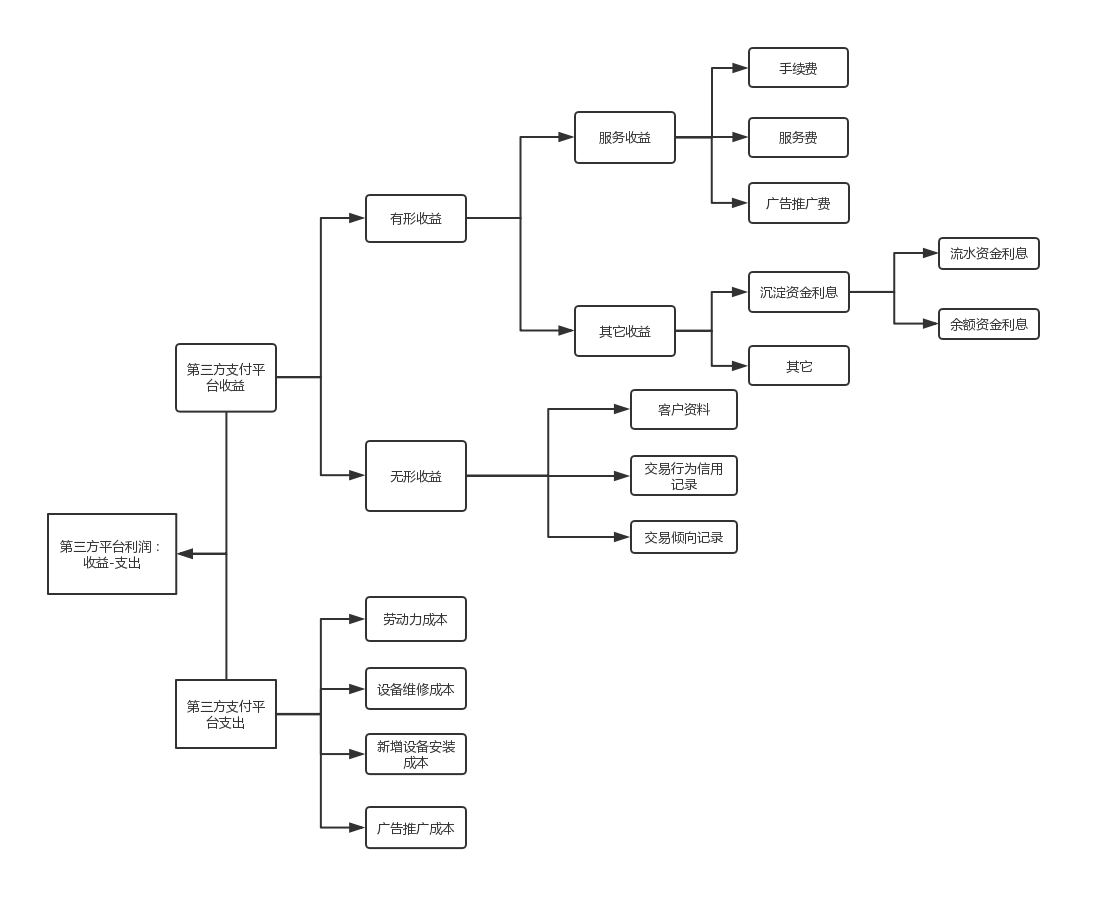
\includegraphics[scale=0.4]{profit.png}
\caption{盈利模型}
\end{figure}
现从以下四个方面构建收入模型:

1.手续费$T_1$:即第三方向用户收取手续费和向银行支付的手续费之差,无论是,线上支付的支付宝,还是线下支付的拉卡拉,手续费都是第三方支付平台的传统盈利方式。附件三中对手续费的区间描述为$0.08\%-1.25\%$,根据微信,支付宝等主流第三方支付平台的手续费率,在模型中取手续费率$FreeRate=0.1\%$。可得手续费$t_1$的表达式为:
\begin{equation}
T_1=S_{sum}*FreeRate
\end{equation}

2.服务费$T_2$:这里所指的服务费是指第三方支付平台为其客户提出支付解决方案,提供支付系统以及各种增值服务。这也应该是第三方支付平台最核的盈利模式。支付宝服务费为$0.6\%$,在模型中取服务费率$ServiceRate=​0.6\%$,可得服务费$T_2$表达式为:
\begin{equation}
T_2=S_{sum}*ServiceRate
\end{equation}

3.广告费$T_3$:为第三方平台向商户收取的广告费用。通过调查广告网站设定广告单价$adFree=40RMB/CPM$,单位为每一千人浏览广告的价格。广告费$T_3$的表达式为:
\begin{equation}
T_3=Pay_{sum}*adFree/1000
\end{equation}

4.沉淀资金$T_4$:沉淀资金即为备付金,其中风险准备金至少为$10\%$,在以活期存款满足日常业务需要之后,可以转成为期三个月的定期存款。协议存款率为$4\%\sim5\%$,手续费估算为$0.78\%$,沉淀金包含长期沉淀金与短期沉淀金两个部分。长期沉淀金主要为用户在第三方平台的余额,而短期沉淀金为第三方平台的流水金额。

沉淀资金增长率的计算:设$r_1$为风险准备金比例,$a_1$为活期资金占总资金比例,$r_2$为三个月的活期年利率,$r_3$为协定年利率。沉淀资金的增长率
\begin{equation}
r=(1-r_1)(a_1*r_2+(1-a_1)*r_3)/12
\end{equation}

设$a_3$为发卡额的保有比例,则沉淀资金的初始值$SedMoney(0)$的表示:
\begin{equation}
SedMoney(0)=(\overline {remian} * {NumberOfPeople})*a_3
\end{equation}

设第i月的沉淀资金经过$j$月以后的总额为$SedMoney^j(i)$,则$SedMoney^j(i)$的表达式为
\begin{equation}
SedMoney^j(i)=\left\{
\begin{aligned}
 & (1+r)*(1-t_1)SedMoney(i) &j=1\\
 & (1+r)*(1-t_1)SedMoney^{j-1}(i) &j=3n-2&&j != 1\\
&(1+r)*SedMoney^{j-1}(i)  & j=3n-1or3n\\
\end{aligned}
\right.
\end{equation}

计算沉淀资金的年利润:
\begin{equation}
T_4=\sum_{i=0}^{11} SedMoney^{12-i}(i)-\sum_{i=0}^{11} SedMoney(i)
\end{equation}

\subsubsection{第三方支付平台的支出}
将平台的支出分为固定成本和推广成本

1. 固定成本$O_1$:主要体现为新增设备安装成本、维护设备成本以及劳动力成本三个部分。

设平均一台支付机器的价格为$V_{machine}$,机器数量为$N_{machine}$,机器维护均价为$V_{maintain}$员工工资支出为$S$,$O_1$的表达式为:
\begin{equation}
O_1=N_{machine}*(V_{machine}+V_{maintain})+S
\end{equation}

2. 推广费用$O_2$:主要体现为平台在各个媒体渠道投放广告用来提高平台的知名度以及市场份额

设投放广告数量为$N_{ad}$,广告均价为$V_{ad}$,$O_2$的表达式为:
\begin{equation}
O_2=N_{ad}*V_{ad}
\end{equation}

\subsubsection{第三方支付平台的盈利模型}
第三方平台的总盈利$W$:收入-支出
\begin{equation}
W=T_1+T_2+T_3+T_4-O_1-O_2
\end{equation}

结合表达式$1\sim10$可得:
\begin{equation}
\begin{split}
W=&S_{sum}*FreeRate+S_{sum}*ServiceRate+Pay_{sum}*adFree/1000\\&+\sum_{i=0}^{11} SedMoney^{12-i}(i)-\sum_{i=0}^{11} SedMoney(i)\\&-(N_{machine}*(V_{machine}+V_{maintain})+S)-N_{ad}*V_{ad}
\end{split}
\end{equation}

\subsubsection{问题二模型的求解}
\subsubsection{问题二模型的分析}
\subsection{问题三的建模与解答}

\subsubsection{问题三模型的建立}


\subsubsection{问题三模型的求解与分析}


\section{模型的评价}
\subsection{模型的优点}
\subsection{模型的缺点}
\subsection{灵敏度分析}
\subsection{模型的改进}
\section{模型的推广与应用}

\begin{figure}
\begin{minipage}[t]{0.5\linewidth}
\centering
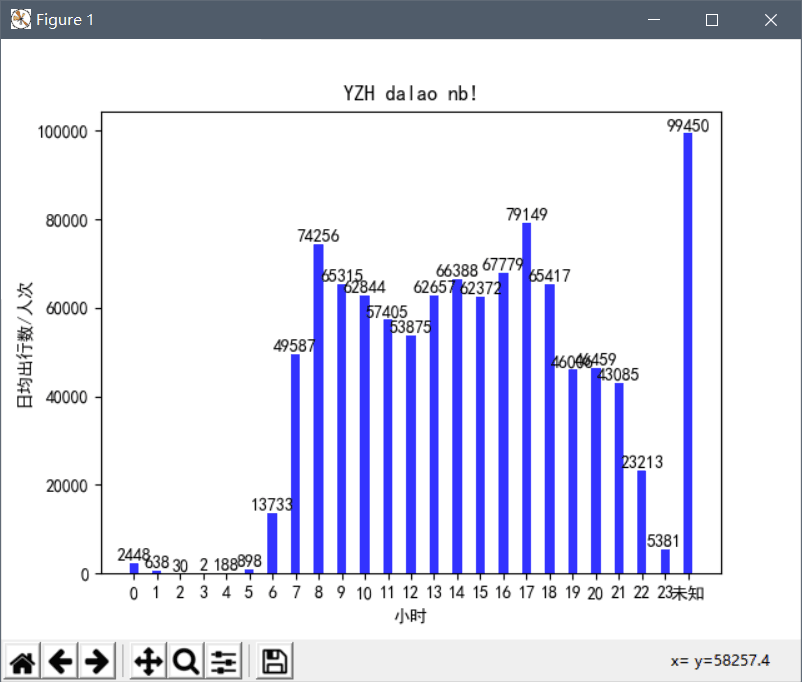
\includegraphics[width=2.2in]{chart.png}
\caption{fig1}
\label{fig:side:a}
\end{minipage}%
\begin{minipage}[t]{0.5\linewidth}
\centering
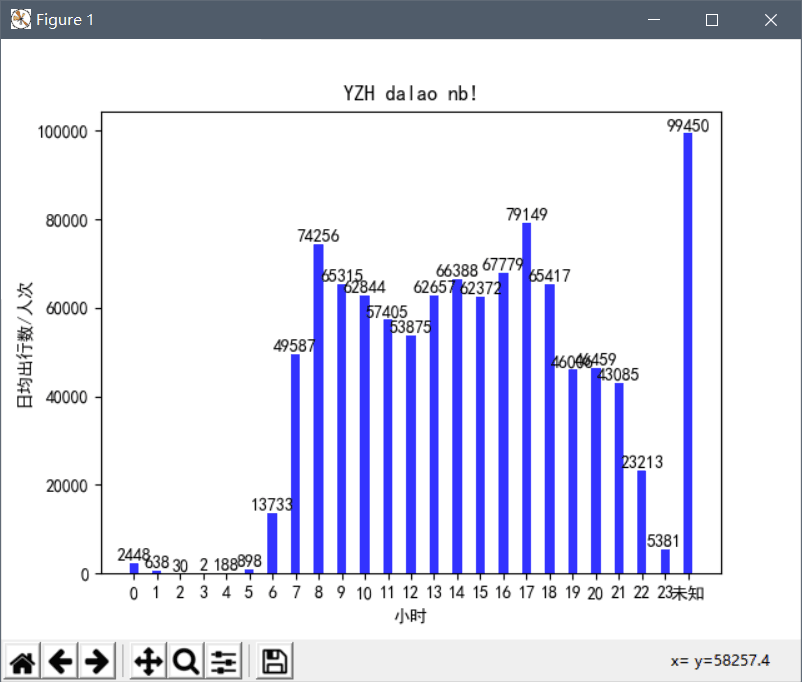
\includegraphics[width=2.2in]{chart.png}
\caption{fig2}
\label{fig:side:b}
\end{minipage}
\end{figure}

\begin{figure}[htbp]
\centering
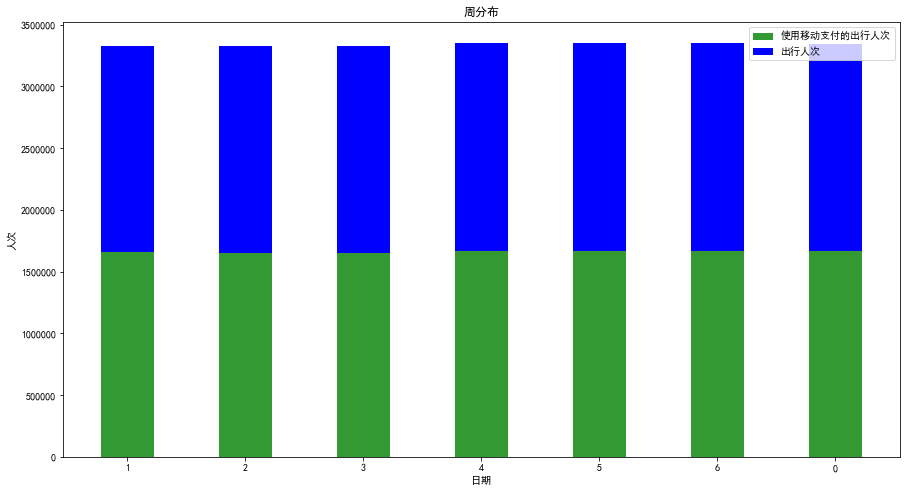
\includegraphics[scale=0.5]{indexw.png}
\caption{图}
\end{figure}

\begin{figure}[htbp]
\centering
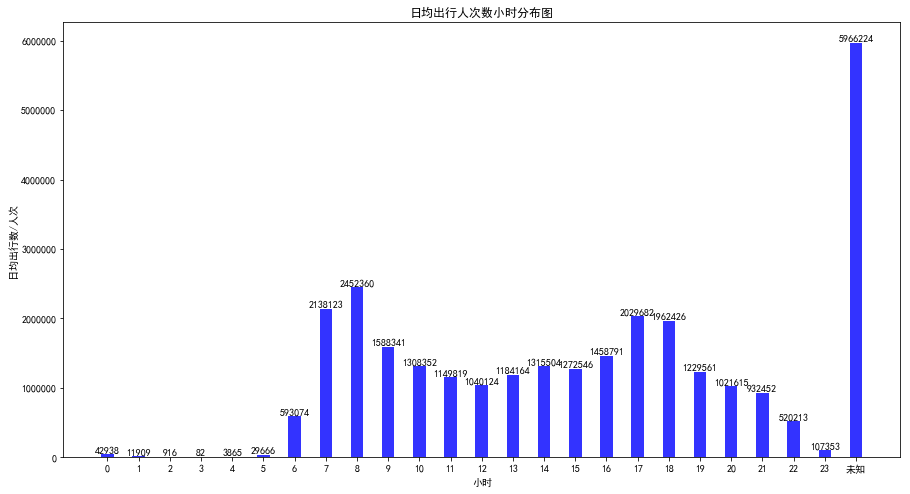
\includegraphics[scale=0.5]{index.png}
\caption{日均出行人次小时分布图}
\end{figure}

\begin{figure}[htbp]
\centering
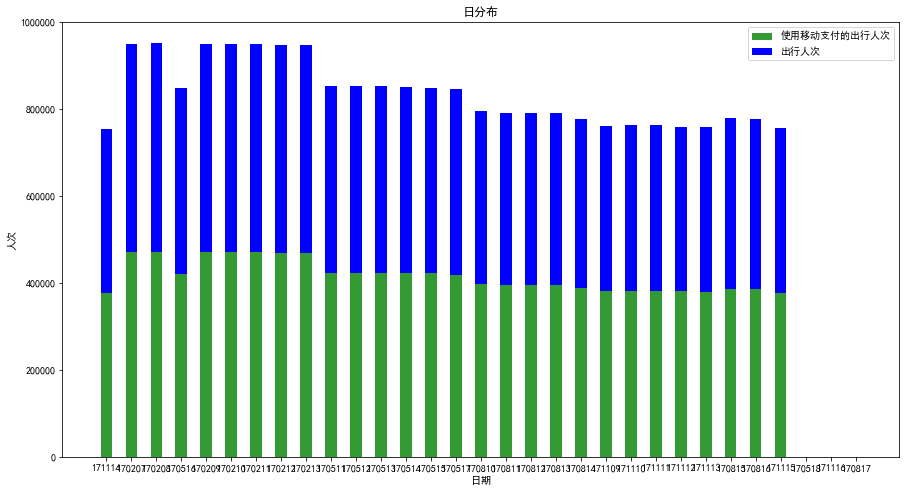
\includegraphics[scale=0.5]{indexed.png}
\caption{图}
\end{figure}
%参考文献
\begin{thebibliography}{9}%宽度9
 \bibitem{bib:one} 王琛.第三方支付的主要盈利模式及存在的风险分析——以支付宝为例[J].商业文化,2015(18):166-168.
 \bibitem{bib:two}钱凯凯,蒋秀.从支付宝微信支付看第三方支付的盈利模式[J].商场现代化,2016(30):77-78.
 \bibitem{bib:three}孙吉贵,刘杰,赵连宇.聚类算法研究[J].软件学报,2008(01):48-61.
 \bibitem{bib:four}陈佳琪. 第三方支付平台的风险评估[D].湖南大学,2018.
 \bibitem{five}姚宁. 基于移动平台的第三方支付模式研究[D].华东理工大学,2016.
 \bibitem{bib:six}张念,王毅磊.中国移动支付发展的现状及问题——以支付宝为例[J].现代营销(下旬刊),2019(03):50.
 \bibitem{bib:seven}易涌征. 移动支付消费者接受的影响因素研究[D].浙江大学,2012.
 
\end{thebibliography}

\newpage
%附录
\begin{appendices}
\section{遗传算法--python 源程序}
\begin{lstlisting}[language=python]
print helloworld!
 \end{lstlisting}
 \section{程序--X代码}
\begin{lstlisting}[language=c]
cout<<"helloworld";
 \end{lstlisting}
\end{appendices}

\end{document} 